\newcommand{\figuraSolucionesLaneEmden}{%
\begin{figure}[H]
    \centering
    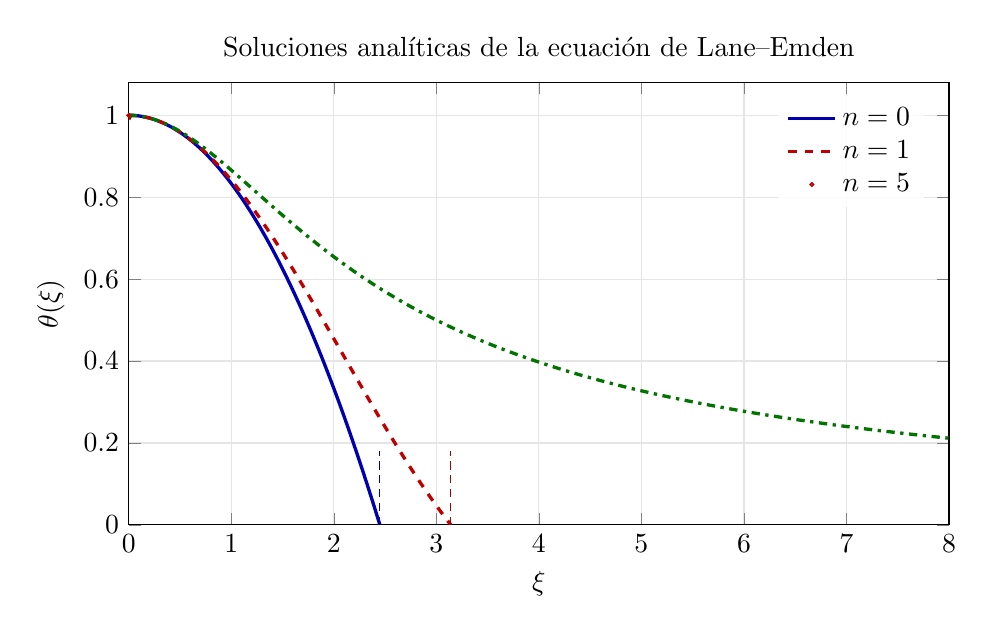
\begin{tikzpicture}
        \begin{axis}[
            width=12cm,
            height=7.2cm,
            xmin=0,xmax=8,
            ymin=0,ymax=1.08,
            xlabel={$\xi$},
            ylabel={$\theta(\xi)$},
            title={Soluciones analíticas de la ecuación de Lane--Emden},
            grid=major,
            grid style={gray!20},
            legend style={at={(0.97,0.97)},anchor=north east,
                          draw=none,fill=white,fill opacity=0.85,
                          text opacity=1}]

            \addplot[very thick,blue!70!black,domain=0:sqrt(6),samples=120]
                {1-x^2/6};
            \addlegendentry{$n=0$}

            \addplot[very thick,red!75!black,dashed,domain=0.001:pi,samples=160]
                {sin(deg(x))/x};
            \addplot[only marks,mark=*,mark size=0.7pt,red!75!black]
                coordinates {(0,1)};
            \addlegendentry{$n=1$}

            \addplot[very thick,green!45!black,dash dot,domain=0:8,samples=180]
                {1/sqrt(1+x^2/3)};
            \addlegendentry{$n=5$}

            \draw[densely dashed,blue!60!black]
                (axis cs:{sqrt(6)},0)--(axis cs:{sqrt(6)},0.18);
            \draw[densely dashed,red!65!black]
                (axis cs:{pi},0)--(axis cs:{pi},0.18);
        \end{axis}
    \end{tikzpicture}
    \caption{Soluciones regulares para $n=0$, $n=1$ y $n=5$. Los dos
    primeros politropos tienen radio finito, mientras que la solución con
    $n=5$ se aproxima a cero únicamente cuando $\xi\to\infty$.}
    \label{fig:soluciones-lane-emden}
\end{figure}%
}